%!TEX root = ..\lections.tex
Осциллятор – простейшая динамическая система с двумерным фазовым
пространством. Несмотря на простоту, с помощью этой системы можно описать
важнейшие колебательные процессы: периодические, затухающие и
нарастающие. Круг реальных задач, приводящих к модели в виде
осциллятора,чрезвычайно широк и имеет самую разнообразную природу.
Например, к таким задачам относятся различные механические устройства, в
которых происходит взаимодействие масс и упругих сил, электрические
контуры, содержащие ёмкостные и индуктивные компоненты, некоторые виды
акустических резонаторов, простейшие популяционные задачи и др. Изучение
динамических свойств осцилляторов мы начнём с задач, в которых нелинейные
механизмы отсутствуют или пренебрежимо малы.

\section{Динамика линейного осциллятора}%
\label{sec:5.1}

Рассмотрим электрический контур, состоящий из последовательно соединённый ёмкости $C$, индуктивности $L$ и сопротивления $R$ (см. рис.\ref{fig:5.1}а).
Обозначим через $q$ заряд конденсатора $C$. Согласно закону Кирхгофа
\begin{equation}
        \label{eq:5.1}
        u_r + u_1 + u_c =0,
\end{equation}

\begin{figure}[h!]
        \centering
        \begin{minipage}{0.45\linewidth}
                \centering  
                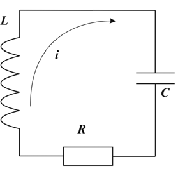
\includegraphics[]{fig/lect5/1a}

                (a)
        \end{minipage}
        \begin{minipage}{0.45\linewidth}
                \centering  
                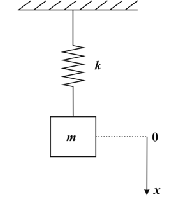
\includegraphics[]{fig/lect5/1b}

                (b)      
        \end{minipage}
        \caption{Линейные осцилляторы: электрический контур (а); груз массы $m$ на пружине с жёсткостью $k$, совершающий малые колебания около положения равновесия (b).}
        \label{fig:5.1}
\end{figure}
т.е. сумма падений напряжения на элементах контура равна нулю, поскольку в цепи отсутствуют внешние источники напряжения. Пусть $i$-- ток, протекающий в контуре, который, как известно, связан с зарядом $q$ следующим образом
\begin{equation}
        \label{eq:5.2}
        i = \dv{q}{t}.
\end{equation}
Тогда для напряжение на элементах контура можно записать
\begin{equation}
        \label{eq:5.3}
        u_R = Ri = R \dv{q}{t}, ~ u_L = L \dv{i}{t} = L \dv[2]{q}{t},~ u_C= \frac{q}{C}.
\end{equation}
Подставляя \eqref{eq:5.3} в \eqref{eq:5.1}, получим уравнение
\begin{equation}
        \label{eq:5.4}
        L\dv[2]{q}{t} + R \dv{q}{t} + \frac{q}{C} = 0.
\end{equation}
Перепишем уравнение \eqref{eq:5.4}, для удобства дальнейшего изложения, в следующем эквивалентном виде
\begin{equation}
        \label{eq:5.5}
        \ddot x + 2 \delta x + \omega_0^2 x =0,
\end{equation}
где 
\begin{equation}
        \label{eq:}
        2 \delta = \frac{R}{L}, ~ \omega_0^2=\frac{1}{LC}.
\end{equation}
Реальные системы, динамика которых описывается уравнением \eqref{eq:5.5}, принято называть
\textbf{линейными осцилляторами}. Уравнение \eqref{eq:5.5} содержит два параметра, имеющих ясный смысл: $\omega_0$--частота собственных колебаний, а параметр $\delta$ характеризует потери в системе.

Другим примером линейного осциллятора может служить груз на пружине (см. рис.\ref{fig:5.1}b), совершающий малые колебания вблизи положения равновесия при наличии силы трения пропорциональной скорости $\dot x$. Динамика такой системы также описывается уравнением \eqref{eq:5.5}, в котором $x$ -- смещение груза из положения равновесия.

\subsection{Гармонический осциллятор}%
\label{sub:5.1.1}

Предположим, что в изолированной физической системе отсутствует
рассеяние энергии, вызванное переходом энергии движения в тепловую
энергию. В таких идеализированных системах запас энергии остаётся
постоянным, и они называются \textbf{консервативными} .

Покажем, что системы, динамика которых описывается уравнением \eqref{eq:5.5}    
при $\delta = 0$, является консервативными, и выясним основные свойства таких
систем. При $\delta = 0$ представим уравнение \eqref{eq:5.5} в виде
\begin{equation}
        \label{eq:5.6}
        \begin{cases}
                \dot x = y, \\
                \dot y = - \omega_0^2 x.
        \end{cases}
\end{equation}
Очевидно, что система \eqref{eq:5.6} имеет единственное состояние равновесия в начале координат, корни характеристического уравнения которого имеют вид: $\lambda_{1,2} = \pm i \omega_0$. Следовательно (см. \ref{lect3}), это состояние равновесия является центом,и на фазовой плоскости $(x,y)$ любая траектория, отличная от состояния
равновесия, представляет собой замкнутую кривую. Уравнение
соответствующих интегральных кривых без труда можно найти из системы
 \eqref{eq:5.6} путём её сведения к уравнению первого порядка с разделяющимися
переменными 
\begin{equation}
        \label{eq:5.7}
        \frac{y^2}{2} + \omega^2 \frac{x^2}{2} = C, C= \const\geq0.
\end{equation}
Из \eqref{eq:5.7} следует, что нетривиальные интегральные кривые системы \eqref{eq:5.6} имеют вид эллипсов, оси которых совпадают с координатными осями. На фазовой плоскости $(x,y)$ согласно первому уравнению
в \eqref{eq:4.6} переменная $x$ вдоль траекторий возрастает при $y>0$ и убывает при $y<0$ (см. рис.\ref{fig:4.2}а). Найдём время $T$, за которое изображающая точка совершит один полный оборот вдоль произвольной замкнутой траектории, стартующей с произвольных начальных условий
\begin{equation}
        \label{eq:5.8}
        x(0) = x_0,~ y(0) = y_0 . 
\end{equation}
Запишем общее решение уравнение \eqref{eq:5.6}
\begin{equation}
        \label{eq:5.9}
        \begin{cases}
                x = C_1 \cos(\omega_o t) + C_2 \sin(\omega_0t), \\
                y = - \omega_0 C_1 \sin(\omega_0t) +\omega_0C_2\cos(\omega_0t),
        \end{cases}
\end{equation}
где $C_{1,2}= \const$. Из \eqref{eq:5.8}, \eqref{eq:5.9} находим уравнение искомой траектории
\begin{equation}
        \label{eq:5.10}
        \begin{cases}
                x=x_0 \cos(\omega_0t) + \frac{y_0}{\omega_0} \sin(\omega_0)
                y = -x_0\omega_0\sin(\omega_0t) + y_0\cos(\omega_0t). 
        \end{cases}
\end{equation}
Очевидно, что в момент $t=T$  должны выполняться условия
\begin{equation}
        \label{eq:5.11}
        x(T) = x_0, ~ y(T)=y_0.
\end{equation}
Подставляя \eqref{eq:5.10} в \eqref{eq:5.11}, получим систему линейных относительно $\sin(\omega_0 T)$ и $\cos(\omega_0t)$ уравнений
 \begin{equation}
        \label{eq:5.12}
        \begin{cases}
                x_0 \cos(\omega_0 T) + \frac{y_0}{\omega_0} \sin(\omega_0 T) = x_0\\
                y_0 \cos(\omega T) - x_0\omega_0 \sin(\omega_0 T) = y_0.
        \end{cases}
\end{equation}

\begin{figure}[h!]
        \centering
        \begin{minipage}{0.45\linewidth}
                \centering  
                
\includegraphics[]{fig/lect5/2a}

                (a)
        \end{minipage}
        \begin{minipage}{0.45\linewidth}
                \centering  
                
\includegraphics[]{fig/lect5/2b}

                (b)      
        \end{minipage}
        \caption{Фазовый портрет гармонического осциллятора (а); гармонические колебания периода
        $T =  \frac{2\pi}{\omega}~ (b)$.}
        \label{fig:5.2}
\end{figure}
Решая систему \eqref{eq:5.12} обычным образом, находим, что

\begin{equation}
        \label{eq:}
        \cos(\omega_0T) = 1, \quad \sin(\omega_0 T) =0
\end{equation}
следовательно,
\begin{equation}
        \label{eq:5.13}
        T= \frac{2\pi}{\omega_0}.
\end{equation}
Представим для удобства решение \eqref{eq:5.10} в виде
\begin{equation}
        \label{eq:5.14}
        x= A\cos(\omega_0 t+ \phi) \\
        y = -A\omega_0\sin(\omega_0t +\phi),
\end{equation}
где 
\begin{equation}
        \label{eq:}
        A= \sqrt{ x_0^2 + \frac{y_0^2}{\omega_0^2}}, \quad \tg{ \phi} = \frac{\omega_0x_0}{y_0}.
\end{equation}
Из \eqref{eq:5.13}, \eqref{eq:5.14} вытекает, что осциллятор \eqref{eq:5.9} при любых начальных условиях
совершает \textbf{ синусоидальные (гармонические) } колебания с амплитудой $A$, фазой $\phi$ и частотой $\omega_0$, независящей от начальных условий (см. рис.\ref{fig:5.2}b). Осциллятор \eqref{eq:5.6} называется гармоническими, а совершаемые им колебания, период которых не зависит от начальных условий, -- \textbf{ изохронными}.
При этом уравнение \eqref{eq:5.7} представляет собой закон сохранения энергии, поскольку первое слагаемое в \eqref{eq:5.7} есть кинетическая

\begin{equation}
        \label{eq:5.15}
        E_K = \frac{y^2}{2} = (A^2 \omega_0^2 \cos^2(\frac{\omega_0 t + \phi)}{2},
\end{equation}
а второе -- потенциальная энергия осциллятора
\begin{equation}
        \label{eq:5.16}
        E_{\text{П}} = \frac{x^2}{2} = (A^2 \omega_0^2 \sin^2(\frac{\omega_0t + \phi)}{2}.
\end{equation}
Из \eqref{eq:5.7}, \eqref{eq:5.15} и \eqref{eq:5.16} следует, что полная энергия осциллятора остаётся при колебаниях постоянной
\begin{equation}
        \label{eq:}
        E = E_K + E_{\text{П}} = \const,
\end{equation}
однако переходит из одного вида в другой.

Поясним теперь связь между траекториями на фазовой плоскости осциллятора \eqref{eq:4.6} и колебаниями в реальном пространстве. Это соотношение иллюстрирует рис.\ref{fig:5.3}, на котором представлена замкнутая фазовая траектория осциллятора \eqref{eq:5.6}, описывающего малые колебания груза на пружине (рис.\ref{fig:5.1}b), и четыре состояния груза в пространстве, соответствующие различным точкам фазовой траектории. 
\begin{figure}[h!]
        \centering
        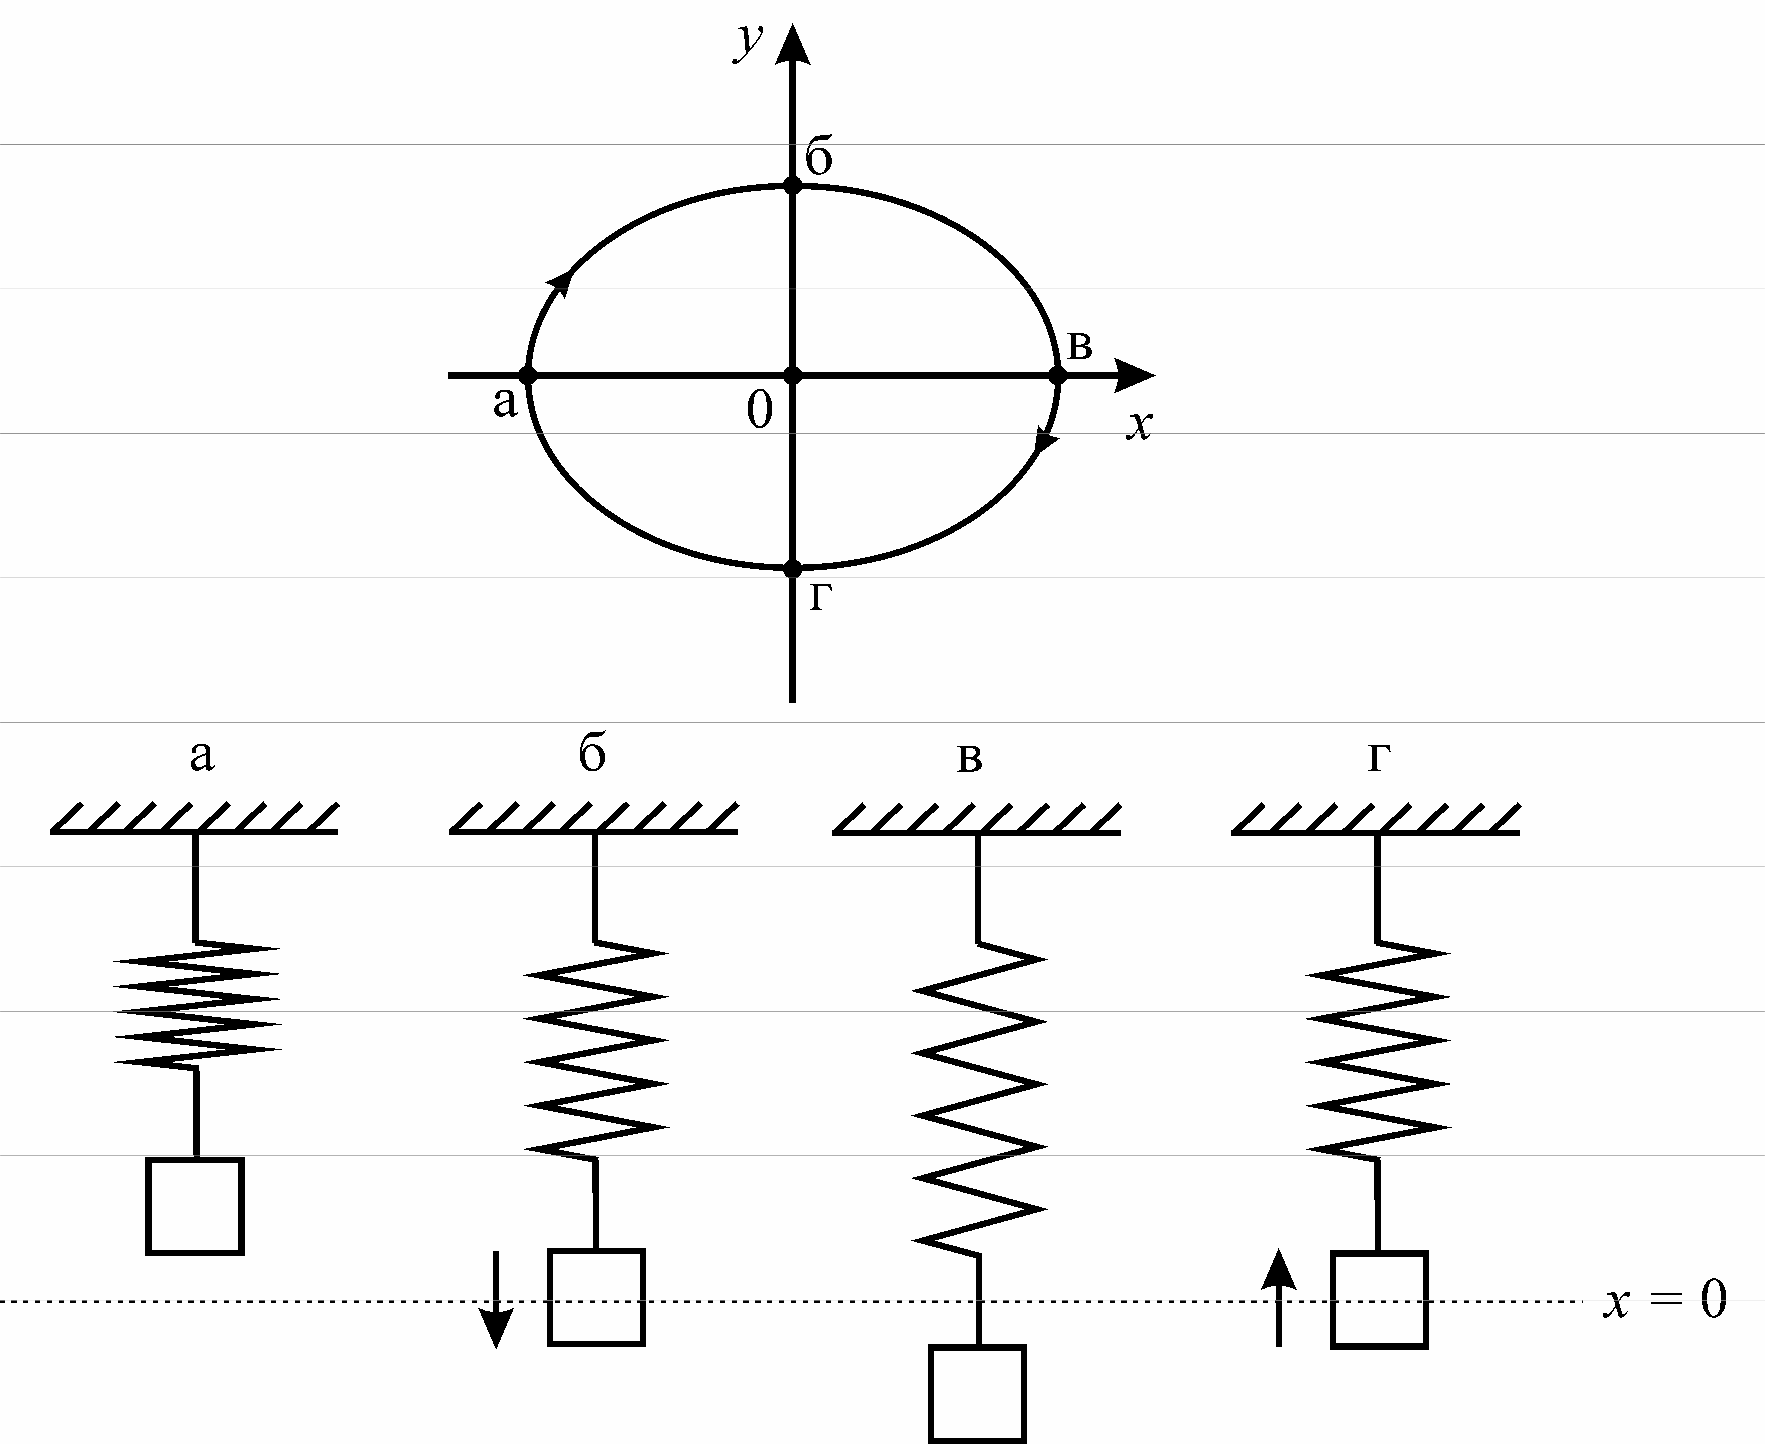
\includegraphics[width=0.6\linewidth]{fig/lect5/3}
        \caption{Фазовая траектория осциллятора \eqref{eq:5.6} и четыре различных состояния груза на пружине  }
        \label{fig:5.3}
\end{figure}


\subsection{Линейный осциллятор при наличии потерь}%
\label{sub:5.1.2}

В реальных системах всегда происходит рассеяние (диссипация) энергии,
её потери, вызванные наличием элементов, трансформирующих энергию
движения в тепловую. Например, в электрическом контуре это омическое
сопротивление, а в случае груза на пружине – сила трения (рис.\ref{fig:5.1}). Если
диссипация энергии в системе (линейной или нелинейной) ничем не
компенсируется, то с течением времени любые колебания затухают и система
приходит в равновесное состояние. Такие системы называют диссипативными
динамическими системами (см. лекцию \ref{lect1}), и их динамика принципиально
отличается от динамики консервативных систем.

Рассмотрим динамику простейшей диссипативной системы -- линейного осциллятора \eqref{eq:5.5} при $\delta \neq 0$. Перепишем \eqref{eq:5.5} в виде системы
\begin{equation}
        \label{eq:5.17}
        \dot x = y, \\
        \dot y = -2 \delta y - \omega_0^2 x.
\end{equation}
На фазовой плоскости $(x,y)$ система \eqref{eq:5.17} имеет единственное состояние равновесия $O(x=0,y=0)$, характеристическое уравнение для которого имеет вид
\begin{equation}
        \label{eq:5.18}
        \lambda^2 + 2 \delta \lambda + \omega_0^2 = 0 
\end{equation}
Динамика двумерных линейных систем полностью определяются типом состояний равновесия (см. лекцию 
\ref{lect3}). Поэтому, анализируя корни уравнения \eqref{eq:5.18}, можно установить возможные колебательные процессы в линейном осцилляторе \eqref{eq:5.17}.

\paragraph{Затухающий процесс.}%
\label{par:zatukhaiushchii_protsess_}

Пусть параметры системы \eqref{eq:5.17} удовлетворяют условиям
\begin{equation}
        \label{eq:5.19}
        \delta > 0, \delta^2 < \omega_0^2.
\end{equation}
Поскольку $\Re \lambda_{1,2} = - \delta < 0 $ состояние равновесия $O$ является устойчивым фокусом
(см. лекцию \ref{lect3}, траекториям которого отвечают осцилляторно затухающие колебания. Фазовый портрет систем \eqref{eq:5.17} представлен на рис.\ref{fig:5.4}а. Траектории пересекают ось абсцисс так, что касательные к ним в точках пересечения имеют вертикальный наклон, поскольку $\dot x =0$, если $y=0$. Кроме того,
\begin{equation}
        \label{eq:}
        \dot y =0, \text{ если } y= - \frac{\omega_0^2}{2\delta}x
\end{equation}
и, следовательно, траектории пересекают эту прямую так, что в точках пересечение наклон касательных к траекториям является горизонтальным. Линии на фазовой плоскости, на которых касательные к траекториям имеют один и тот же наклон называют
\textbf{изоклинами}
соответствующего наклона. В случае системы \eqref{eq:5.17} ось абцисс -- изоклина вертикальных, а прямая $y = - \frac{\omega_0^2}{2\delta}x$-- горизонтальных наклонов.

Исследуем характеристики осцилляторно затухающего процесса. Аналогично \eqref{eq:5.10}, запишем уравнение траектории осциллятора \eqref{eq:5.17}, удовлетворяющей начальным условиям $x(0) = x_0, y(0) = y_0$ 
\begin{equation}
        \label{eq:5.21}
        \begin{cases}
                x=e^{-\delta t} \qty[ x_0 \cos( \omega t) + \frac{y_0- \delta x_0}{\omega} \sin(\omega t) ] ,\\
                y= e^{-\delta t} \qty[\cos(\omega t) - \frac{( -\omega^2 + \delta^2) x_0 + \delta y_0}{\omega} \sin(\omega t)],
        \end{cases}
\end{equation}
или
\begin{equation}
        \label{eq:5.22}
        \begin{cases}
                x = A e^{-\delta t} \sin(\omega t + \phi),\\
                y = i \sqrt{ \delta^2 + \omega^2} A e^{-\delta t} \sin(\omega t + \phi +  \theta),
        \end{cases}
\end{equation}
где 
\begin{equation}
        \label{eq:}
        A = \sqrt{ x_0^2 + \frac{( y_0 + \delta x_0)^2}{\omega^2}}, ~ \tg \phi = \frac{x_0 \omega}{y_0 + \delta x_0}, ~ \tg \theta = - \frac{\omega}{\delta}.
\end{equation}
Из \eqref{eq:5.22} следует, что колебательные процессы, описываемые системой \eqref{eq:5.17} при выполнении условий \eqref{eq:5.19}, являются непериодическими и осцилляторно затухающими. Затухание колебаний происходит по экспоненциальному закону, т.е. на плоскости $(t,x)$ экстремумы функции $x(t)$ лежат на экспонентах $x= \pm A e^{-\delta t}$ (см. рис.\ref{fig:5.3}b). Интервал между любыми двумя соседними экстремумами равен $T = \frac{ 2 \pi}{\omega}$.
Благодаря этому свойству, можно ввести величину, характеризующую скорость затухания осцилляторного процесса -- логарифмический декремент затухания $d$. Пусть $x_1(t_1)$ и $x_2(t_2), t_2>t_1$ -- значение двух соседних экстремумов, например максимумов, т.е.
\begin{equation}
        \label{eq:}
        x_1(t_1) = A e^{- \delta t_2}, \quad x_2(t_2) = A e^{-\delta t_2}.
\end{equation}
Найдем их отношение
\begin{equation}
        \label{eq:5.23}
        \frac{x_1(t_1)}{x_2(t_2)} = e ^{\delta(t_2-t_1)} = e^{\delta T} = e^{\frac{\delta2 \pi}{\omega}}.
\end{equation}
Декремент характеризует убывание амплитуды колебаний во времени, т.е. число $\frac{1}{d}$ равно числу колебаний, после которого амплитуда уменьшится в $e $ раз. Заметим, что этот закон затухания колебания выполняется во-первых, если система является линейной, а во-вторых, если потери энергии происходят линейно относительно $\dot x$. Нарушение этих условий делает соотношение \eqref{eq:5.23}не справедливым и использование декремента для характеристики  процесса требует специальных оговорок.

\begin{figure}[h]
        \centering
        \begin{minipage}{0.45\linewidth}
                \centering  
                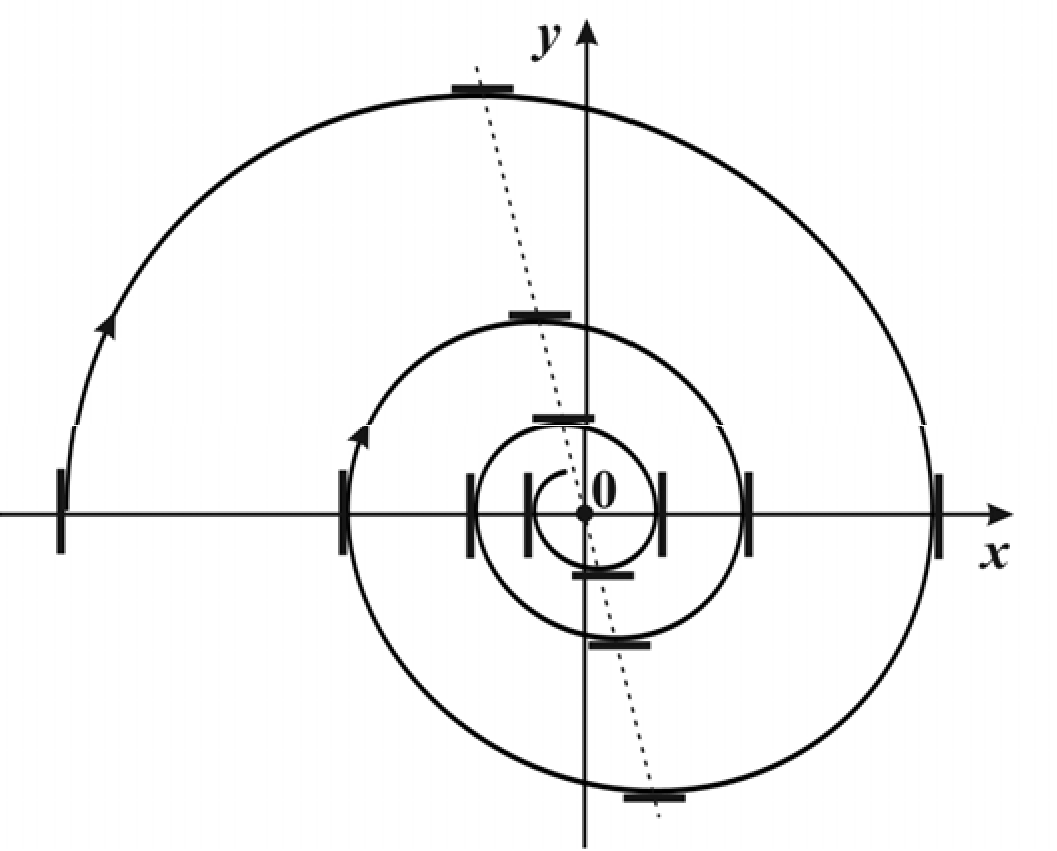
\includegraphics[]{fig/lect5/4a}

                (a)
        \end{minipage}
        \begin{minipage}{0.45\linewidth}
                \centering  
                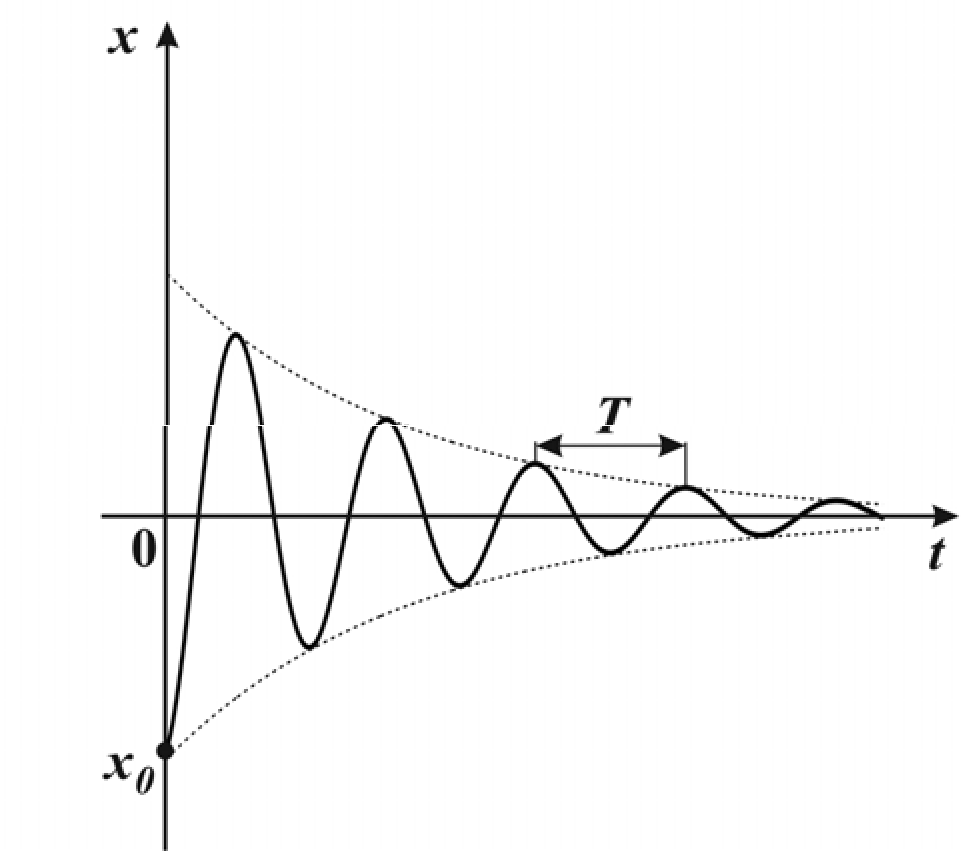
\includegraphics[]{fig/lect5/4b}

                (b)      
        \end{minipage}
        \caption{Устойчивый фокус, пунктирной линией показана изоклина горизонтальных наклонов (а); осцилляторно затухающие колебания (b). }
        \label{fig:5.4}
\end{figure}



\paragraph{Затухающий апериодический процесс.}%
\label{par:zatukhaiushchii_aperiodicheskii_protsess_}

Предположим, что параметры системы \eqref{eq:5.17} удовлетворяют условиям
\begin{equation}
        \label{eq:5.24}
        \delta>0,~ \delta^2 > \omega_0^2
\end{equation}
При выполнении \eqref{eq:5.24} состояние равновесия $O$ имеет отрицательные корни характеристического уравнения
\begin{equation}
        \label{eq:5.25}
        \lambda_{1,2} = - \delta \pm \sqrt{ \delta^2 - \omega_0^2}
\end{equation}
и, следовательно, является устойчивым узлом (см. рис.\ref{fig:5.5}а) каждой траекторий которого отвечает затухающий апериодический процесс осциллятора. Несмотря на то, что при всех начальных условиях наблюдается однотипное поведение осциллятора, некоторая, не принципиальная, разница в характере установления равновесного состояния всё-таки существует. Эта разница определяется расположением начальных условий на фазовой плоскости относительно 
ведущего и неведущих направлений узла (см. лекцию \ref{lect3}). Для узла $O$ эти направления задаются соответственно уравнениями
\begin{equation}
        \label{eq:5.26}
        y= \lambda_1 x, ~ y=\lambda_2 x.
\end{equation}
Прямые \eqref{eq:5.26} делят фазовуб плоскость на четыре области (см. рис.\ref{fig:5.5}а). Для начальных условий из областей 2, 4 апериодически затухающие процессы характеризуются монотонным изменением переменных $x(t)$, $y(t)$, а из области 1, 3 -- наличием экстремумов в моменты времени, когда траектории пересекают ось абсцисс (см. рис.\ref{fig:5.5}). 
\begin{figure}[h]
        \centering
        \begin{minipage}{0.45\linewidth}
                \centering  
                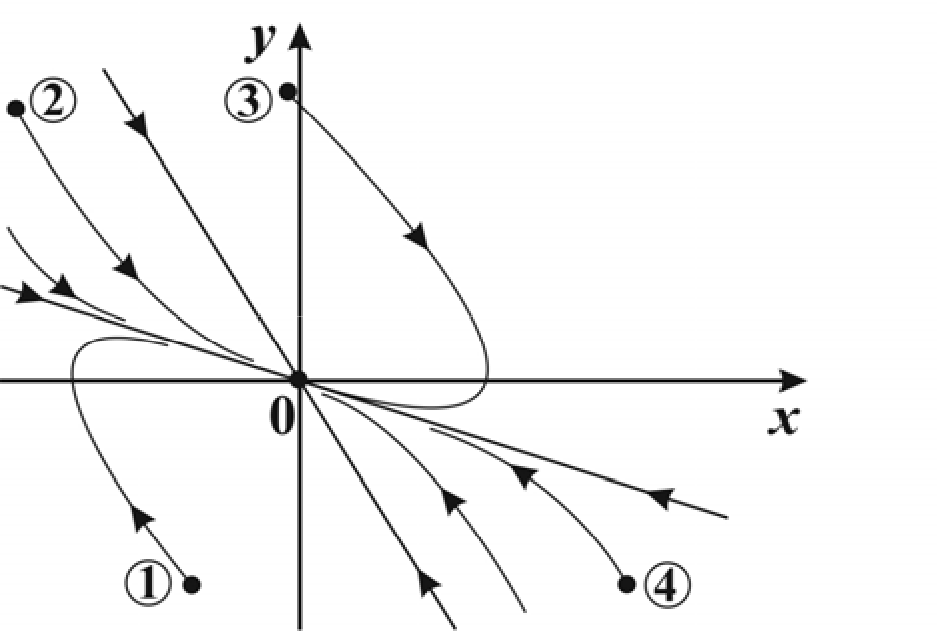
\includegraphics[]{fig/lect5/5a}

                (a)
        \end{minipage}
        \begin{minipage}{0.45\linewidth}
                \centering  
                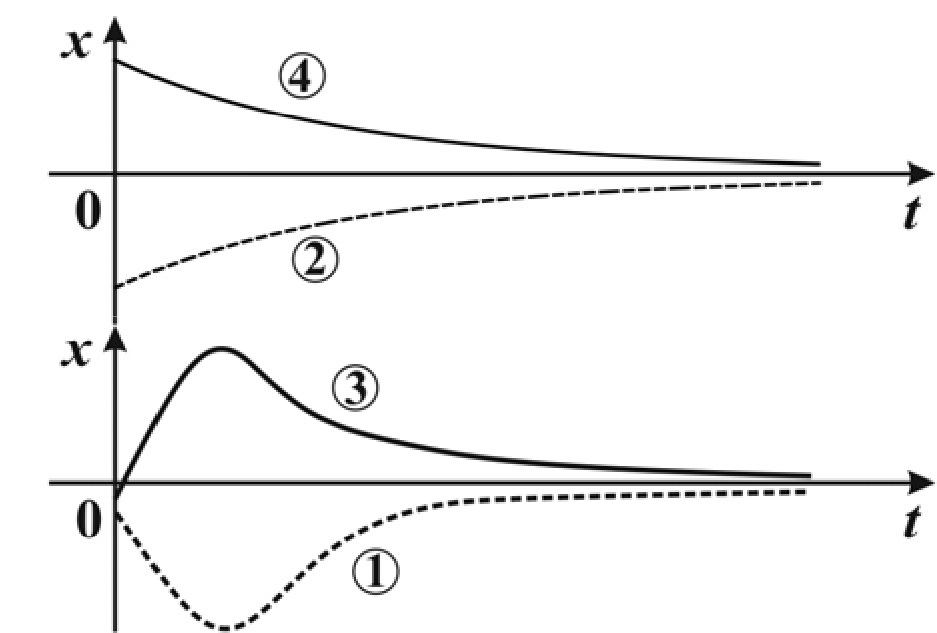
\includegraphics[]{fig/lect5/5b}

                (b)      
        \end{minipage}
        \caption{Устойчивый узел (а); апериодические затухающие процессы, соответствующие начальным условиям из области 1-4 (b).}
        \label{fig:5.5}
\end{figure}

\subsection{Линейный осциллятор с <<отрицательным>> затуханием}%
\label{sub:5.1.3}

Пусть в системе \eqref{eq:5.17} теперь параметр $\delta<0$. Рассмотрим изменение во времени полной энергии осциллятора, задаваемой уравнениями \eqref{eq:5.15}, \eqref{eq:5.16}. В силу системы \eqref{eq:5.17} имеем
\begin{equation}
        \label{eq:5.27}
        \pdv{E}{t} = y \dot y + \omega_0^2 x \dot x = - 2\delta y^2
\end{equation}
Поскольку $\delta<0$ из \eqref{eq:5.27} следует, что энергия $E$ во времени растёт. Понятно, что для этого осциллятор должен пополнять энергию из вне, так как собственного источника энергии у него нет. В некоторых системах (так называемых активных) за счёт внешних источников энергии возможно формирование таких динамических процессов с <<отрицательным>> затуханием (трением) или <<отрицательным>> сопротивлением, приводящих к временному росту энергии.
Примерами подобных систем являются: в радиоэлектронике -- устройства,
содержащие элементы, у которых вольт-амперные характеристики имеют
падающие участки, в механике --  системы, в которых силы трения имеют
нелинейную, с падающим участком, зависимость от относительной скорости
трущихся поверхностей (например, маятники на вращающихся валах) и др.
Динамика таких систем в окрестности равновесных состояний приближённо
может быть описана с помощью системы \eqref{eq:5.17} при $\delta<0$.

Рассмотрим динамику системы \eqref{eq:5.17} при $\delta<0$. В этом случае из \eqref{eq:5.20} и \eqref{eq:5.25} следует, что состояние равновесия является неустойчивым фокусом если $\delta^2<\omega_0^2$ (см. рис.\ref{fig:5.6}а) или неустойчивым узлом, если $\delta^2 \geq \omega_0^2$ (см. рис.\ref{fig:5.6}b). Следовательно, при $\delta<0$ осциллятор \eqref{eq:5.27} описывает нарастающие колебания,
примеры которых даны на рис.\ref{fig:5.6}c и рис.\ref{fig:5.6}d. 
\begin{figure}[h]
        \centering
        \begin{minipage}{0.45\linewidth}
                \centering  
                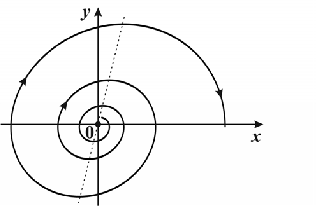
\includegraphics[]{fig/lect5/6a}

                (a)
        \end{minipage}
        \hfill
        \begin{minipage}{0.45\linewidth}
                \centering  
                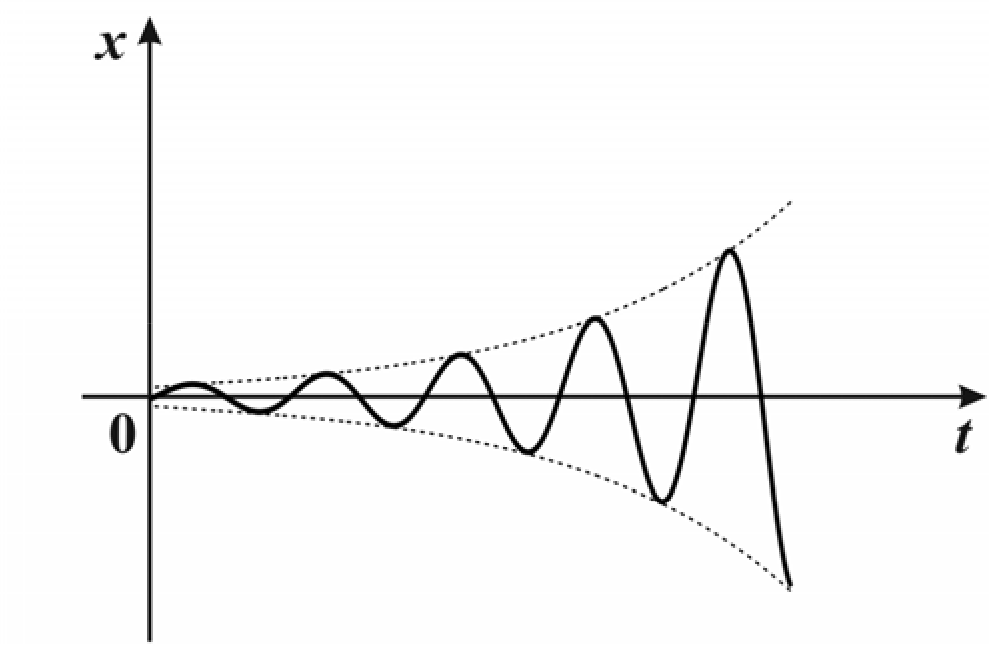
\includegraphics[]{fig/lect5/6b}

                (b)      
        \end{minipage}
        \vfill
        \begin{minipage}{0.45\linewidth}
                \centering  
                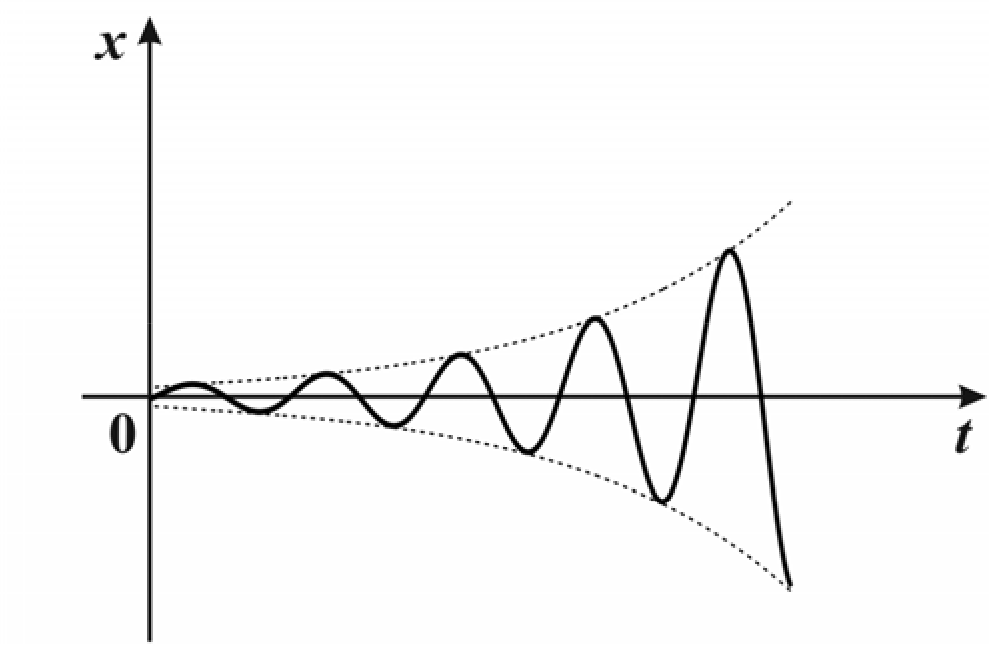
\includegraphics[]{fig/lect5/6c}

                (c)
        \end{minipage}
        \hfill
        \begin{minipage}{0.45\linewidth}
                \centering  
                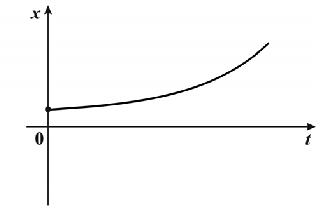
\includegraphics[]{fig/lect5/6d}

                (d)      
        \end{minipage}
        \caption{Неустойчивый фокус (а); неустойчивый узел (b); осцилляторно нарастающий процесс (c); апериодический нарастающий процесс (d).}
        \label{fig:5.6}
\end{figure}
В случае фокуса колебание
нарастают по экспоненциальному закону (рис. \ref{fig:5.6}c), который характеризуется
так называемым логарифмическим \textbf{инкрементом нарастания}
$\delta_1= -\delta$,
применяемым без оговорок лишь для линейных систем. В случае узла вид
нарастающих колебаний зависит от позиции на фазовой плоскости начальных
условий относительно ведущего и неведущего направлений, т.е. может
происходить как монотонно (\ref{fig:5.6}c), так и не монотонно (с одним
экстремумом) во времени.

Таким образом, <<отрицательное>> трение (потери) приводят к
неограниченному росту колебаний, что, конечно, не может происходить в
реальных системах. Этот рост является следствием линейной идеализации
задачи и, как мы увидим в дальнейшем, нелинейные механизмы его
ограничивают.

\section{Динамика нелинейного осциллятора}%
\label{sec:5.2}

Как мы уже отмечали, линейные системы представляют собой
простейшие, идеализированные модели реальных процессов. Даже сильно
упрощённые модели реальных систем, как правило, являются нелинейными.
Например, незначительное изменение условий задач, рассмотренных в разделе
\ref{sec:5.1}, приводит к модели в виде уже нелинейного осциллятора. Так, если в задаче
о колебаниях груза (рис.\ref{fig:5.1}b) не ограничиваться малыми смещениями, то сила с
которой пружина действует на груз будет нелинейной функцией смещения и
осциллятор становится нелинейным. Другим примером нелинейного
осциллятора может служить электрический контур, представленный на
рис.\ref{fig:5.1}а, в случае, если ёмкость $C$ содержит сегнетоэлектрик.
\subsection{Консервативный нелинейный осциллятор}%
\label{sub:5.2.1}

Предположим, что рассеяние энергии в реальной системе происходит
очень медленно – например, груз на пружине помещён в среду с очень малым
трением, в электрическом контуре отсутствует сопротивление $R$, а омическое
сопротивление соединительных проводов пренебрежимо мало и так далее.
Ясно, что этом случае диссипативные механизмы, обеспечивающие рассеяние
энергии, не окажут сильного влияния (на не слишком больших временных
интервалах) на динамику системы и ими можно пренебречь. Другими словами,
можно считать, что в этом случае система является консервативной. Основной
моделью таких систем является консервативный осциллятор, динамика
которого описывается уравнением
\begin{equation}
        \label{eq:5.28}
        \ddot x + f(x) = 0,
\end{equation}
где $f(x)$ -- нелинейная функция. В частности, к уравнению вида \eqref{eq:5.28} могут быть сведены упомянутые выше осцилляторы. Представим для удобства уравнения \eqref{eq:5.28} в виде системы
\begin{equation}
        \label{eq:5.29}
        \begin{cases}
                \dot x = y, \\
                \dot y = -f(x).
        \end{cases}
\end{equation}
Прежде всего, покажем, что динамика системы \eqref{eq:5.29} является консервативной. Поделив второе уравнение системы \eqref{eq:5.29} на первое и разделив переменные, имеем
\begin{equation}
        \label{eq:5.30}
        y \dd{y} = - f(x) \dd{x}.
\end{equation}
Проинтегрируем уравнение \eqref{eq:5.30} от некоторого начального момента $t=t_0$ до произвольного момента времени $t$. В результате получим
\begin{equation}
        \label{eq:5.31}
        \frac{y^2}{2} - \frac{y_0^2}{2} = - \int\limits_{x_0}^{x} f(x) \dd{x}, 
\end{equation}
где $x_0 = x(t_0),~ y_0=y(t_0)$. Нетрудно видеть, что уравнение \eqref{eq:5.31} можно переписать в следующем виде
\begin{equation}
        \label{eq:5.32}
        \frac{y^2}{2} + \int\limits_{0}^{x_0} f(x) \dd{x} = h, 
\end{equation}
где
\begin{equation}
        \label{eq:5.33}
        h=\frac{y_0^2}{2} + \int\limits_{0}^{x_0}  f(x) \dd{x}.
\end{equation}
Из \eqref{eq:5.33} следует, что $h = \const$ и представляет собой полную энергию осциллятора \eqref{eq:5.29} в момент $t= t_0$. В левой же части уравнения \eqref{eq:5.32} стоит полная энергия осциллятора в момент $t$, состоящая из суммы
кинетической $E_K$  потенциальной $E_{\text{П}}$ энергии, где
\begin{equation}
        \label{eq:5.34}
        E_K = \frac{y^2}{2}, \quad E_{\text{П}} = \int\limits_{0}^{x} f(x) \dd{x}. 
\end{equation}
Таким образом, с одной стороны уравнение \eqref{eq:5.32} задаёт закон сохранения энергии, а с другой -- в неявном виде уравнение интегральных кривых, отвечающих данному $h$. Заметим, что, если для данного $h$ из \eqref{eq:5.32} найти действительных значений $(x,y)$ не удаётся, то это означает, что энергия осциллятора \eqref{eq:5.29} не может принимать такого значения.

Покажем теперь как, используя уравнение \eqref{eq:5.32}, можно построить фазовый портрет системы \eqref{eq:5.29}.

Предварительно приведём некоторые свойства траекторий, вытекающие непосредственно из системы \eqref{eq:5.29} и уравнения \eqref{eq:5.32}. Из \eqref{eq:5.29} следует, что координаты состояний равновесия этой системы определяются системой
\begin{equation}
        \label{eq:5.35}
        y=0, \quad f(x)=0
\end{equation}
и, следовательно, они расположены на оси абсцисс. При этом, так как $\dot x = 0$ при $y=0$ во всех точках оси абсцисс, отличных от состояний равновесия, касательные к траекториям имеют вертикальный наклон, то есть ось абсцисс на этих участках является изоклиной вертикальных наклонов. Кроме того, поскольку уравнение \eqref{eq:5.32} инвариантно относительно замены $y \to -y$, то фазовые траектории системы \eqref{eq:5.29} симметричны относительно оси абсцисс. 
Поэтому достаточно установить вид траекторий лишь на верхней полуплоскости, а поведение траекторий при $y<0$
 можно найти, используя свойство симметрии.

 Рассмотрим теперь процедуру построения фазового портрета системы \eqref{eq:5.29} с помощью уравнения \eqref{eq:5.32}. Из \eqref{eq:5.34} вытекает, что
 \begin{equation}
         \label{eq:5.36}
         \pdv{E_{\text{П}}}{x} = f(x)
 \end{equation}
 Следовательно, в состояниях равновесия потенциальная энергия $E_{\text{П}}(x)$ либо достигает экстремума, либо имеет точку перегиба. Проанализируем поведение фазовых траекторий системы
 \eqref{eq:5.29} в окрестности состояний равновесия, соответствующих этим трём случаям. Для этого из \eqref{eq:5.32} выразим $y$ через $E_{\text{П}}(x)$ 
 \begin{equation}
         \label{eq:5.37}
         y = \sqrt{ 2 \qty[ h - E_{\text{П}}(x)] }
 \end{equation}
 Согласно \eqref{eq:5.37} траектории системы \eqref{eq:5.29} соответствующие данному $h$, существуют на фазовой плоскости только для тех $x$, где $E_{\text{П}}(x) \leq h$. Причём, для
 $x$, удовлетворяющих уравнению $E_{\text{П}} = h$ и переменная $y=0$. В силу \eqref{eq:5.37} имеем 
 \begin{equation}
         \label{eq:5.38}
         \dv{y}{x} = - \frac{  \dv{ E_{ \text{П} } } {x}  } 
         {\sqrt{2 \qty[ h - E_{\text{П}}(x) ] }}
 \end{equation}
 Отсюда получаем, ещё одно свойство траекторной системы \eqref{eq:5.29}
 \begin{equation}
         \label{eq:5.39}
         \begin{cases}
                 \dv{y}{x} > 0, & \text{ если } \dv{E_{\text{П} } }{x} < 0, \\
                 \dv{y}{x} < 0, & \text{ если } \dv{E_{\text{П} } }{x} > 0. \\
         \end{cases}
 \end{equation}
 Опираясь на представленные здесь свойства траекторий, можно построить фазовый портрет системы \eqref{eq:5.29}, зная лишь вид функции $E_{\text{П}}(x)$. Рис. \ref{fig:5.7} иллюстрирует методику такого построения в случае, когда $E_{\text{П}}(x)$ имеет локальные минимум, максимум и точку перегиба. Если функция $E_{\text{П}}(x)$ имеет минимум, то на фазовой плоскости система \eqref{eq:5.29} имеет состояние равновесия типа центр (см. рис.\ref{fig:5.7}а), которое устойчиво по Ляпунову. Максимум функции
 $E_{\text{П}}(x)$ соответствует на фазовой плоскости седло (см. рис.\ref{fig:5.7}b). Заметим, что в силу \eqref{eq:5.37} у седла нелинейной системы \eqref{eq:5.29} сепаратрисы имеют вид некоторых кривых, а не прямых, как в случае линейного осциллятора.
 Наконец, если $E_{\text{П}}(x)$ имеет точку перегиба, то на фазовой плоскости существует сложное состояние равновесия (см. рис.\ref{fig:5.7}c), имеющие два нулевых корня характеристического уравнения.

 Изложенный выше приём построения фазового портрета осциллятора \eqref{eq:5.29} справедлив не только для анализа поведение траекторий в окрестности состояний равновесия, но и для построения полного фазового портрета на всей фазовой плоскости. Продемонстрируем это на примере нелинейного осциллятора, описывающего колебание математического маятника.

 Рассмотрим динамику маятника, состоящего из невесомого стержня длины $l$ и груза массы $m$ (см. рис.\ref{fig:5.8}а). Маятник находится в поле силы тяжести и может свободно вращаться в вертикальной плоскости вокруг точки подвеса.

 \begin{figure}[h]
         \centering
         \includegraphics[width=0.6\linewidth]{example-image-a}
         \caption{Три различных вида функции $E_{\text{П}}(x)$ и отвечающие им фазовые портреты системы \eqref{eq:5.29}: состояние равновесия (а); состояние равновесия седло (b); сложное состояние равновесия с двумя нулевыми характеристическими корнями (c).}
         \label{fig:5.7}
 \end{figure}

 Пусть $\phi$ -- угол отклонения маятника от вертикали. Запишем уравнение движения маятника
 \begin{equation}
         \label{eq:5.40}
         J \dv{\omega}{t} = \sum\limits_{k} M_k,
 \end{equation}
 где $J$--момент инерции груза, $J= ml^2$, $\omega = \dv{\phi}{t}$-- угловая скорость массы $m$, $M_k$-- момент сил, действующих на груз. На груз действует две силы -- тяжести и вязкого трения, которая пропорциональна мгновенной скорости и равна -- $k l \dot \phi$, $k>0$. Моменты этих сил будем вычислять относительно оси, проходящей через точку подвеса маятника перпендикулярно плоскости колебаний маятника. Они определяются следующим образом
 \begin{equation}
         \label{eq:5.41}
         M_1 = - mgl \sin \phi, \quad M_2 = - kl^2 \pdv{\phi}{t},
 \end{equation}
 где $g$ -- ускорение свободного падения. Подставляя \eqref{eq:5.41} в \eqref{eq:5.40}, получим
 \begin{equation}
         \label{eq:5.42}
         ml^2 \dv[2]{\phi}{t} = - mgl\sin \phi - kl^2 \dv{\phi}{t}.
 \end{equation}
 \begin{figure}[h]
         \centering
         \includegraphics[width=0.6\linewidth]{example-image-a}
         \caption{Колебательные движения маятника (а), вращательные движения маятника (b); 
         потенциальная функция (c); фазовый портрет осциллятора \eqref{eq:5.43} (d).}
         \label{fig:5.8}
 \end{figure}
 Сделаем в \eqref{eq:5.42} замену времени $t = \sqrt{ \frac{l}{g}} \tau$, в результате которой это уравнение примет вид
 \begin{equation}
         \label{eq:5.43}
         \ddot \phi + \lambda \dot \phi + \sin \phi =0,
 \end{equation}
 где точкой обозначено дифференцирование по $\tau$, а $\lambda = \frac{k}{m} \sqrt{ \frac{l}{g}}$
-- безразмерный параметр, характеризующий диссипативные потери в системе.

Исследуем сначала динамику уравнения \eqref{eq:5.43} в случае отсутствия диссипативных потерь, т.е. в случае $\lambda=0$. При $\lambda=0$ уравнение \eqref{eq:5.43} эквивалентно системе
\begin{equation}
        \label{eq:5.44}
        \begin{cases}
                \dot \phi = y, \\
                \dot y = - \sin \phi.
        \end{cases}
\end{equation}
В силу периодичности по $\phi$ правой части системы \eqref{eq:5.44} её фазовым пространством является цилиндр $G = S^1 \times \R$. Цилиндричность фазового пространства системы \eqref{eq:5.44} имеет ясный физический смысл -- маятник может совершать движения как без вращения (см. рис.\ref{fig:5.8}а),
так и с вращением вокруш точка подвеса (см. рис.\ref{fig:5.8}b). Для построения фазового портрета осциллятора \eqref{eq:5.44} воспользуемся методикой изложенной выше. Рассмотрим потенциальную энергию осциллятора \eqref{eq:5.44} -- $E_{\text{П}}(\phi) = - \cos \phi$. Построив график функции $E_{\text{П}}(x)$ (см. рис.\ref{fig:5.8}c) и расположим под ним развёртку фазового цилиндра, мы без труда получаем
фазовый портрет осциллятора \eqref{eq:5.44} (см. рис.\ref{fig:5.8}d). На цилиндрической фазовой поверхности существуют два состояния равновесия: центр -- $O_1(0,0)$ и седло -- $O_1(\pi,0)$. Сепаратрисы седла делят все остальные нетривиальные траектории на два различных 
континуальных семейства периодических
траекторий. К первому семейству относятся периодические траектории из
области ограниченной сепаратрисами. Эти траектории не охватывают фазовый
цилиндр и определяют колебательные движения маятника, т.е. движения без
проворотов вокруг оси подвеса (рис.\ref{fig:5.8}а). Второе семейство образуют
периодические траектории, охватывающие фазовый цилиндр и отвечающие
вращательным движениям маятника (рис.\ref{fig:5.8}b).

Перейдём к обсуждению свойств колебательных процессов осциллятора
\eqref{eq:5.44}. Заметим, что система \eqref{eq:5.44} легко сводится к одному уравнению с
разделяющимися переменными, которое можно проинтегрировать и получить
точные решения, дающие полную информацию о свойствах колебательных
процессов. Такой путь требует привлечения теории эллиптических интегралов
и эллиптических функций Якоби. Мы поступим по-другому – приведём здесь
лишь качественные рассуждения, основанные на свойствах фазовых
траекторий, которые позволяют, тем не менее, установить основные свойства
колебательных процессов.

Рассмотрим сначала колебательные движения осциллятора, которые
существуют, если начальная энергия $h \in (-1,1)$. Для траекторий, локализованных
в малой окрестности состояния равновесия $O_1$ (начальная энергия близка к
значению $-1$), можно считать в первом приближении, что $\sin \phi \simeq \phi$ и колебания
осциллятора \eqref{eq:5.44} близки к колебаниям линейного осциллятора.
Следовательно, малые (вблизи дна потенциальной ямы) колебания осциллятора
\eqref{eq:5.44} будут периодическими квазисинусоидальными, в которых превалирует
амплитуда с основной частотой $\omega=1$ и периодом $T = 2 \pi$ (см. рис.\ref{fig:5.9}а и рис.\ref{fig:5.10}а).
Пусть теперь, начальная энергия близка к единице. Траектория, отвечающая
такому уровню энергии, включает вблизи седла $O_2$ . Поэтому на этих участках
изображающая точка будет сильно замедлять своё движение, что приводит к
формированию на графике $\phi(t)$ почти горизонтальных плато (рис.\ref{fig:5.8}b). Такие
колебания называются \textbf{кноидальными}. Размер этих плато и период колебаний 
будут тем больше, чем ближе начальная энергия к единице. Действительно, при
$h=1$ сепаратрисы сёдел охватывают фазовый цилиндр, образуя пару
двоякоасимптотических (так называемых \textbf{гомоклинических}) траекторий, время
движения по которым стремится к бесконечности. Отсюда и соображений
непрерывности решений от начальных условий вытекает, что период колебаний
траекторий, отвечающих значениям h вблизи единицы, монотонно растёт с
ростом $h$ и при $h \to 1$ стремится к бесконечности. При этом основная частота
близка к нулю, а амплитуды других гармоник имеют некоторое достаточно
сложное распределение, которое приближённо описывается с использованием
гиперболического косинуса (рис.\ref{fig:5.10}b).
\begin{figure}[h]
        \centering
        \includegraphics[width=0.6\linewidth]{example-image-a}
        \caption{Качественный вид зависимости угловой переменной $\phi(t)$ для различных периодических движений осциллятора \eqref{eq:5.44}: квазисуноидальные колебания (а); кноидальные колебания (b); зависимость $\phi(t)$ для двух вращательных траекторий с положительным вращением $\phi$ (c),(d).}
        \label{fig:5.9}
\end{figure}

Рассмотрим теперь вращательные движения осциллятора \eqref{eq:5.44}, которые
существуют, если начальная энергия превосходит единицу. Непосредственно из
вида фазовых траекторий (рис.\ref{fig:5.10}d) следует, что у таких траекторий
зависимость $\phi(t)$ является непериодической функцией, а переменная $y(t)$
(скорость маятника) изменяется периодически. Аналогичные предыдущему
случаю рассуждения показывают, что для энергии близкой к единице как
зависимость угловой переменной (рис.\ref{fig:5.9c}), так и зависимость скорости $y(t)$
будут содержать близкие к горизонтальным линиям плато. С увеличением $h$ эти
плато уменьшаются (рис.\ref{fig:5.9}d) и для достаточно больших $h$ график $\phi(t)$ близок
прямой. Действительно, рассмотрим полную энергию осциллятора \eqref{eq:5.44}
\begin{equation}
        \label{eq:5.45}
        \frac{y^2}{2} - \cos \phi = h
\end{equation}
Из \eqref{eq:5.45} и системы \eqref{eq:5.44}, например, для вращательных движений при $y>0$, имеем
\begin{equation}
        \label{eq:5.46}
        \dot \phi = \sqrt{ 2 \qty(h+ \cos \phi)} = \sqrt{ 2h \qty( 1 + \frac{1}{h} \cos \phi)}.
\end{equation}
Поскольку косинус ограниченная функция, а коэффициент $\frac{1}{h} \ll 1$, если $h \gg 1$,
то из \eqref{eq:5.46} получаем
\begin{equation}
        \label{eq:}
        \dot \phi \simeq \sqrt{2 h}
\end{equation}
и, следовательно, в этом случае
\begin{equation}
        \label{eq:}
        \phi \simeq \sqrt{2h} t + \phi_0.
\end{equation}

\begin{figure}[h]
        \centering
        \includegraphics[width=0.6\linewidth]{example-image-a}
        \caption{Построенные численно спектры периодических движений осциллятора \eqref{eq:5.44}:
        спектр квазисуидальных (а); спектр апериодических колебаний (b). 
По оси ординат использован логарифмический масштаб, а амплитуда гармоник даны в децибелах.}
        \label{fig:5.10}
\end{figure}

Таким образом, основные динамические свойства консервативного нелинейного осциллятора вида \eqref{eq:5.29} состоят в следующем.
\begin{itemize}
        \item Динамика осциллятора полностью определяет величиной начальной энергии.
        \item Период колебаний зависит от начальных условий, т.е. периодические колебиня нелинейного осциллятора \textbf{неизохронны}.
        \item Форма периодических колебаний может варьироваться в широких пределах -- от квазисинусоидальных до кноидальных.
        \item Возможно одновременное сосуществование нескольких устойчивых (по Ляпунову) состояний равновесия, т.е. возможна \textbf{мультистабильность}.
\item Разделение периодических траекторий на группы с принципиально различными свойствами осуществляется сепаратрисами сёдел.
\end{itemize}

\subsection{Нелинейный осциллятор с диссипацией}%
\label{sub:5.2.2}

Рассмотрим, как изменится динамика нелинейного осциллятора, если
учесть в системе действия диссипативных механизмов. Как и в случае
линейного осциллятора, вклад диссипативных потерь будем учитывать
слагаемым пропорциональным $\dot x$ (см. раздел \ref{sub:5.2.2} и уравнение \eqref{eq:5.43}). При
таком предположении динамика нелинейного осциллятора с диссипацией будет
описываться следующей системой
\begin{equation}
        \label{eq:5.47}
        \begin{cases}
                \dot x = y\\
                \dot y = - \lambda y - f(x),
        \end{cases}
\end{equation}
где $0< \lambda$ -- параметр, характеризующий диссипативные потери. Для исследования динамики системы \eqref{eq:5.47} введём в рассмотрение полную энергию осциллятора \eqref{eq:5.32}
\begin{equation}
        \label{eq:}
        E = \frac{y^2}{2} + \int\limits_{0}^{x} f(x) \dd{x} 
\end{equation}
и рассмотрим её изменения во времени под действием системы \eqref{eq:5.47}. В силу \eqref{eq:5.47}
имеем
\begin{equation}
        \label{eq:5.48}
        \dv{E}{t} = -\lambda y^2 \leq 0.
\end{equation}
\begin{figure}[h]
        \centering
        \includegraphics[width=0.6\linewidth]{example-image-a}
        \caption{Фазовые портреты осциллятора \eqref{eq:5.47}: $O_1$ -- устойчивый фокус (а); $O_1$ -- устойчивый узел (b).}
        \label{fig:5.11}
\end{figure}


